\begin{frame}{La placa de desarrollo MOJO v3}
	\begin{columns}
		\begin{column}{.43\textwidth}
			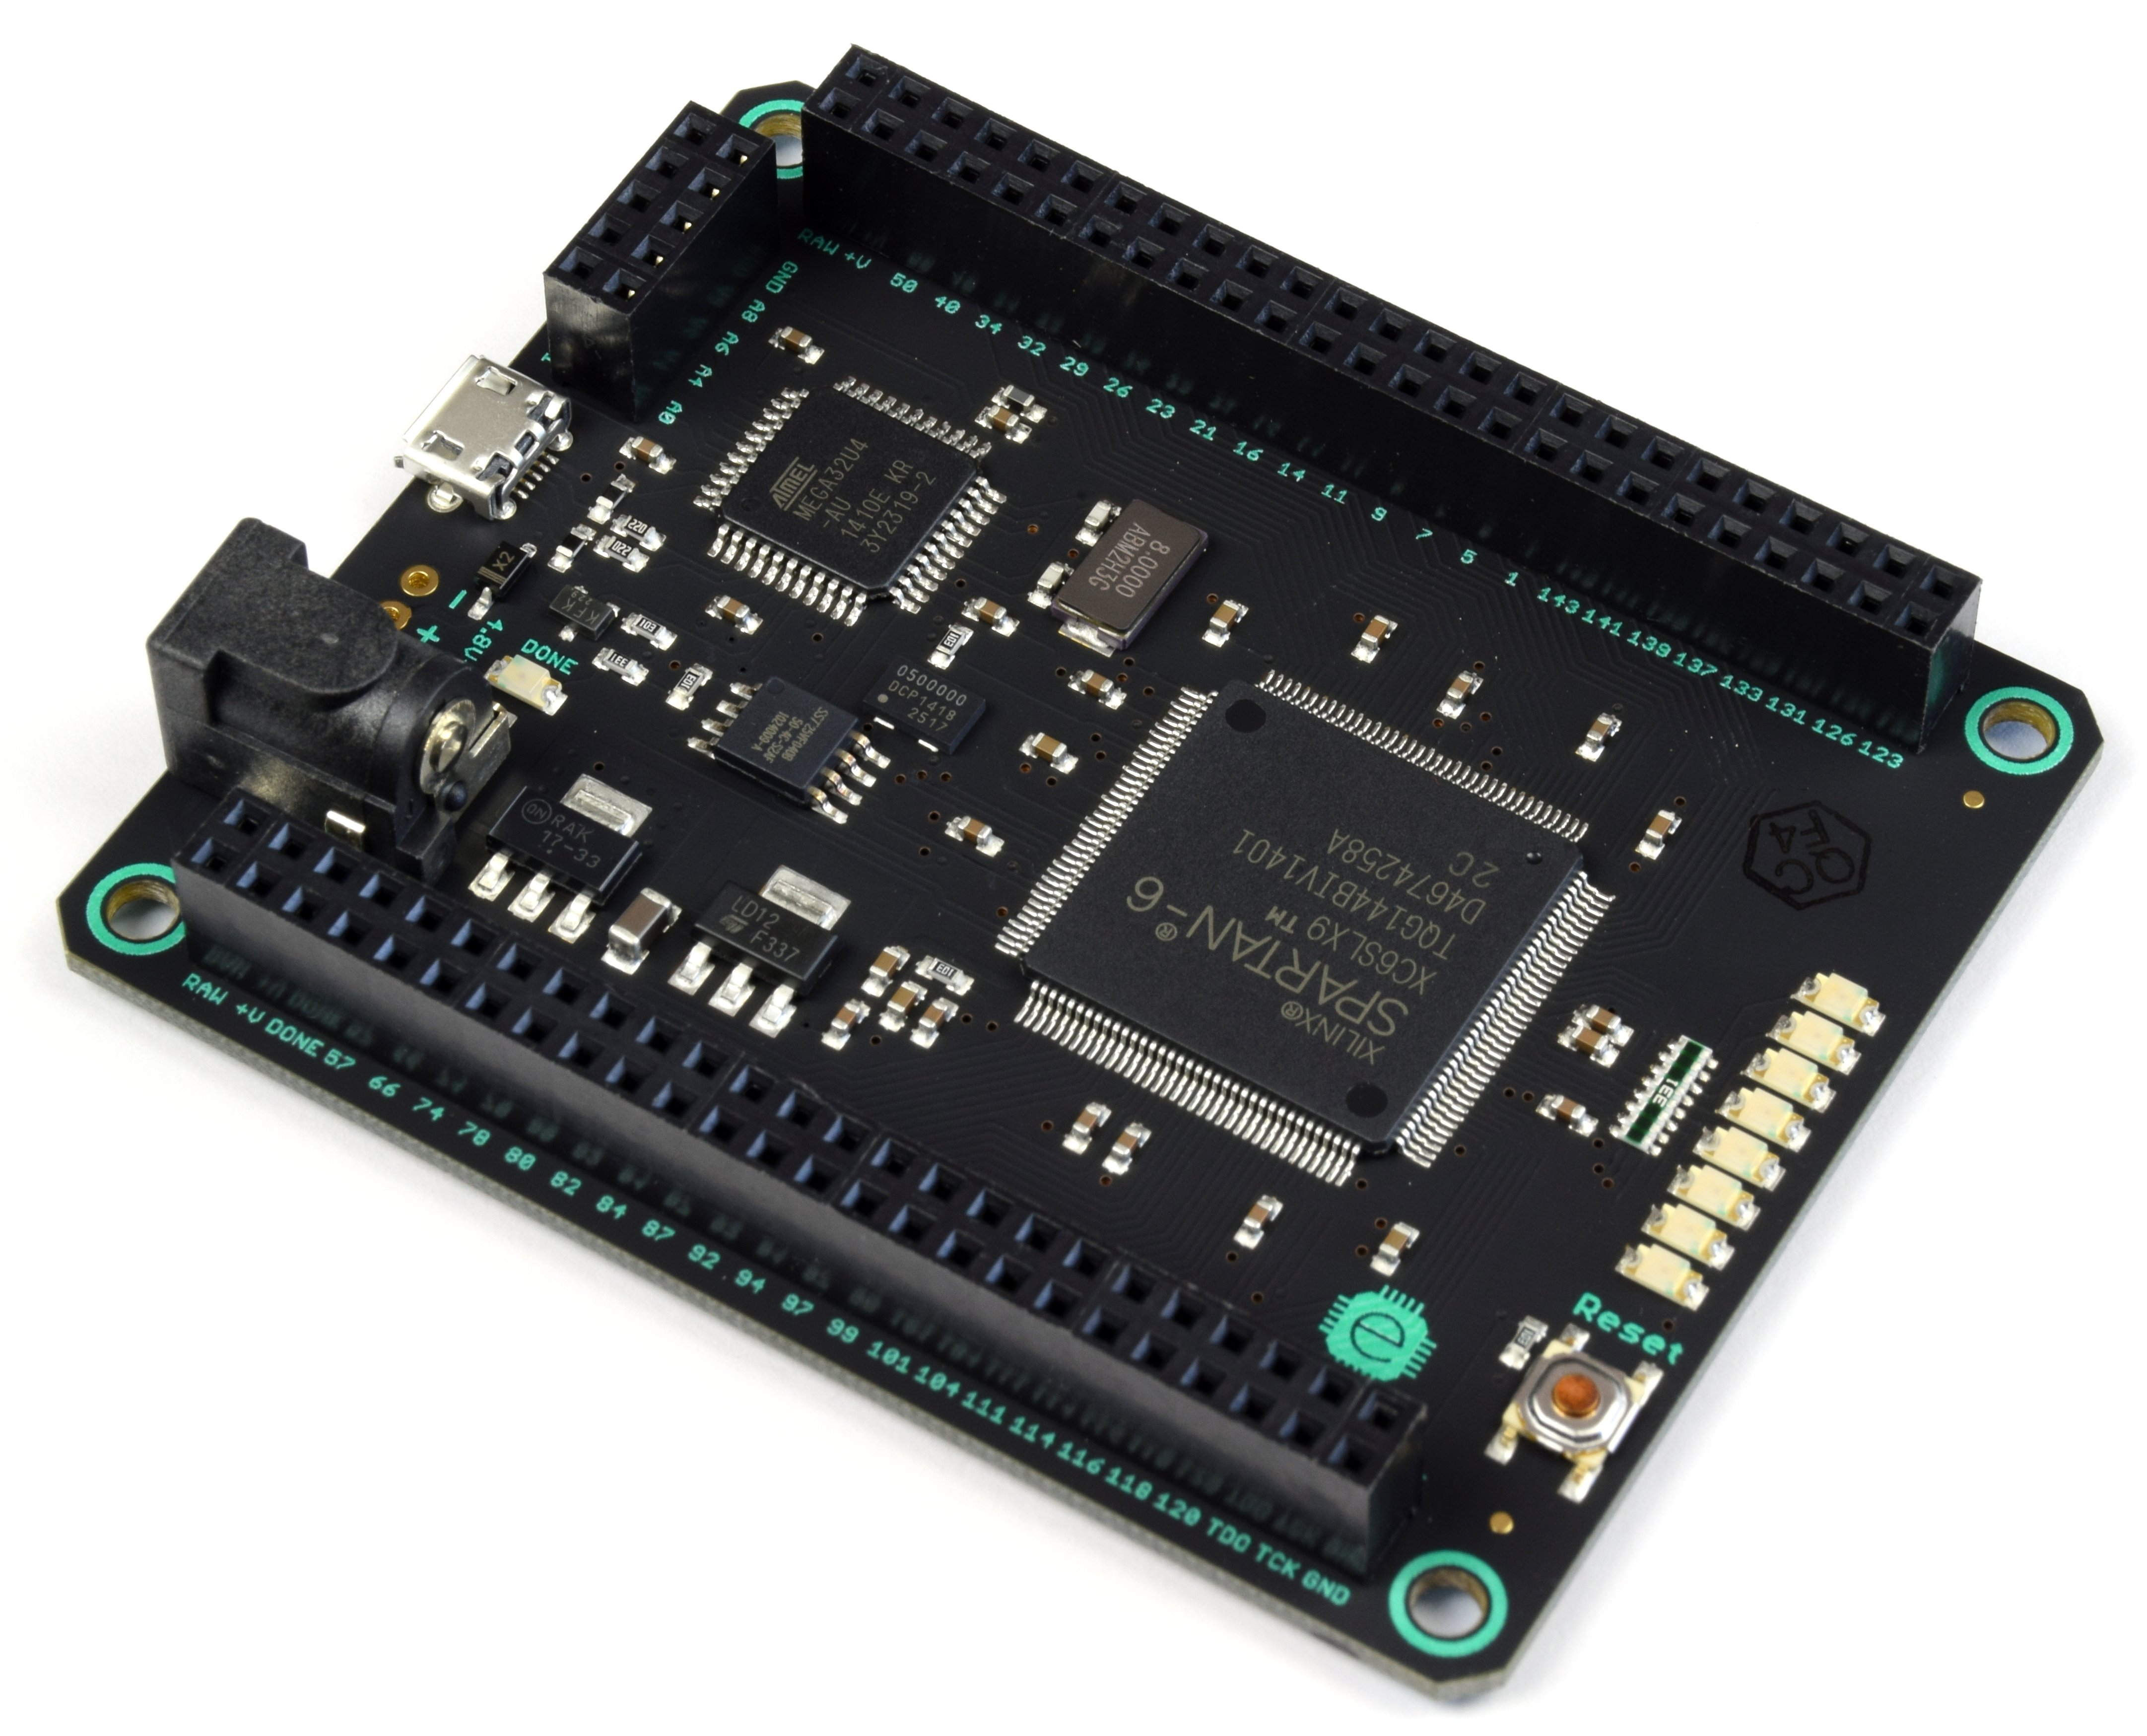
\includegraphics[width=\textwidth]{MojoIso.png}
		\end{column}
		\begin{column}{.55\textwidth}
			\begin{itemize}
				\item FPGA Spartan 6 XC6SLX9 de Xilinx
				\item 84 pines IO digitales
				\item 8 entradas analógicas
				\item 8 LEDs de propósito general
				\item 1 pulsador de propósito general
				\item Regulador de voltaje de entrada de 4.8V - 12V
				\item ATmega32U4 para configurar la FPGA y leer los pines analógicos
				\item Bootloader compatible con Arduino
				\item Memoria flash para almacenar la configuración de la FPGA (programación persistente)
			\end{itemize}
		\end{column}
	\end{columns}
\end{frame}
%\begin{frame}{Estructura interna FPGA}
%	\centering
%	\begin{tikzpicture}[scale=.58]
%		\begin{scope}[transform shape,node distance=5,>=latex,thick]
%			\node[simple]	(cypress)		[]	 			{FIFO Esclava};
%			\node[simple]	(master)	[right=of cypress]	{Maestro Externo};
%			\node[simple,minimum size=70]	(leer)		[right=of master.north west,anchor=north west] {Leer FIFO};
%			\node[simple,minimum size=70]	(escribir)	[right=of master.south west,anchor=south west]	{Escribir FIFO};
%			\node[simple,node distance=8]	(fifo)		[right=of master]	{FIFO Interna (XLNX core generator)};
%			
%			\draw[<->]	([yshift=4*110/6]cypress.east) --node [above]{IFCLK} ([yshift=4*110/6]master.west);
%			\draw[<->]	([yshift=3*110/6]cypress.east) --node [above]{FD[15:0]} ([yshift=3*110/6]master.west);
%			\draw[<-]	([yshift=2*110/6]cypress.east) --node [above]{FIFOADR[1:0]} ([yshift=2*110/6]master.west);
%			\draw[->]	([yshift=1*110/6]cypress.east) --node [above]{EP2\_EMPTY} ([yshift=1*110/6]master.west);
%			\draw[->]	([yshift=0*110/6]cypress.east) --node [above]{EP8\_FULL} ([yshift=0*110/6]master.west);
%			\draw[<-]	([yshift=-1*110/6]cypress.east) --node [above]{SLOE} ([yshift=-1*110/6]master.west);
%			\draw[<-]	([yshift=-2*110/6]cypress.east) --node [above]{SLWR} ([yshift=-2*110/6]master.west);
%			\draw[<-]	([yshift=-3*110/6]cypress.east) --node [above]{SLRD} ([yshift=-3*110/6]master.west);
%			\draw[<-]	([yshift=-4*110/6]cypress.east) --node [above]{PKTEND} ([yshift=-4*110/6]master.west);
%			
%			\draw[<-] (leer) -- node[above]{SLWR} (master.east |- leer);
%			\draw[<-] ([yshift=-1*80/7]leer.east) -- node[above]{EMPTY}([yshift=-1*80/7]fifo.west |- leer);
%			\draw[->] ([yshift=1*80/7]leer.east) -- node[above]{RD\_EN}([yshift=1*80/7]fifo.west |- leer);
%			
%			\draw[<-] (escribir) -- node[above]{SLRD} (master.east |- escribir);
%			\draw[<-] ([yshift=-1*80/7]escribir.east) -- node[above]{FULL}([yshift=-1*80/7]fifo.west |- escribir);
%			\draw[->] ([yshift=1*80/7]escribir.east) -- node[above]{WR\_EN}([yshift=1*80/7]fifo.west |- escribir);			
%			
%			\draw[<-]	([yshift=1*110/6]fifo.west) --node [above]{DIN[15:0]} ([yshift=1*110/6]master.east);
%			\draw[->]	([yshift=0*110/6]fifo.west) --node [above]{DOUT[15:0]} ([yshift=0*110/6]master.east);
%			\draw[<-]	([yshift=-1*110/6]fifo.west) --node [above]{VALID} ([yshift=-1*110/6]master.east);
%			
%			\node[node distance=.4] (fpga) [above=of leer] {FPGA};
%		\end{scope}
%		\begin{scope}[on background layer]
%			\node[rectangle,rounded corners,dashed,fit=(master)(leer)(fpga)(fifo)(escribir),draw=black]{};
%		\end{scope}
%	\end{tikzpicture}
%\end{frame}
\begin{frame}{Interfaz - FPGA}
	\centering
	\begin{tikzpicture}[scale=.7]
		\begin{scope}[transform shape,node distance=4,>=latex,double distance=1.3]
			\node[simple](mef)[]{Maquina de Estados Finitos};
			\node[simple] (fifo) [left=of mef] {FIFO Esclava\\Controlador FX2LP};			
%				\node[simple,minimum size=80](clk)[right=of mef.north east,anchor=north west] {Fuente de reloj};
%				\draw[<-]([yshift=-1*80/3]mef.north east)--node[above]{Reloj}([yshift=-1*80/3]clk.north west);
%				\draw[<-]([yshift=-2*80/3]mef.north east)--node[above]{Reset}([yshift=-2*80/3]clk.north west);

			\node[simple,minimum width=85](interno)[right=of mef]{Sistema\\Implementado en FPGA};
			\draw[double,->]([yshift=5*220/8]mef.south east)--node[above]{Dato\_recibido[15:0]} ([yshift=5*220/8]interno.south west);
			\draw[double,<-]([yshift=4*220/8]mef.south east)--node[above]{Dato\_a\_enviar[15:0]}([yshift=4*220/8]interno.south west);
			\draw[<-]([yshift=3*220/8]mef.south east)--node[above]{Enviar\_datos}([yshift=3*220/8]interno.south west);
			\draw[->]([yshift=2*220/8]mef.south east)--node[above]{SLRD}([yshift=2*220/8]interno.south west);
			\draw[->]([yshift=1*220/8]mef.south east)--node[above]{SLWR}([yshift=1*220/8]interno.south west);	
			\draw[<-]([yshift=-1*220/8]mef.north east)--node[above]{Reloj}([yshift=-1*220/8]interno.north west);
			\draw[<-]([yshift=-2*220/8]mef.north east)--node[above]{Reset}([yshift=-2*220/8]interno.north west);

			\draw[<->,thick] ([yshift=5*110/6]fifo.east) --node [above]{IFCLK} ([yshift=5*110/6]mef.west);
			\draw[<->,thick]	([yshift=4*110/6]fifo.east) --node [above]{FD[15:0]} ([yshift=4*110/6]mef.west);
			\draw[<-,thick]	([yshift=3*110/6]fifo.east) --node [above]{FIFOADR[1:0]} ([yshift=3*110/6]mef.west);
			\draw[->,thick]	([yshift=2*110/6]fifo.east) --node [above]{FLAGA} ([yshift=2*110/6]mef.west);
			\draw[->,thick]	([yshift=1*110/6]fifo.east) --node [above]{FLAGB} ([yshift=1*110/6]mef.west);
			\draw[->,thick]	([yshift=0*110/6]fifo.east) --node [above]{FLAGC} ([yshift=0*110/6]mef.west);
			\draw[->,thick]	([yshift=-1*110/6]fifo.east) --node [above]{FLAGD} ([yshift=-1*110/6]mef.west);
			\draw[<-,thick]	([yshift=-2*110/6]fifo.east) --node [above]{SLOE} ([yshift=-2*110/6]mef.west);
			\draw[<-,thick]	([yshift=-3*110/6]fifo.east) --node [above]{SLWR} ([yshift=-3*110/6]mef.west);
			\draw[<-,thick]	([yshift=-4*110/6]fifo.east) --node [above]{SLRD} ([yshift=-4*110/6]mef.west);
			\draw[<-,thick]	([yshift=-5*110/6]fifo.east) --node [above]{PKTEND} ([yshift=-5*110/6]mef.west);
		\end{scope}
		\begin{scope}[]
			\node[draw=blue,dashed,rectangle,fit={(mef)(interno)},label=north:FPGA,rounded corners]{};
		\end{scope}
	\end{tikzpicture}
\end{frame}

\begin{frame}{Operaciones en la FIFO}
	\framesubtitle{Escritura Asíncrona}
	\only<1>{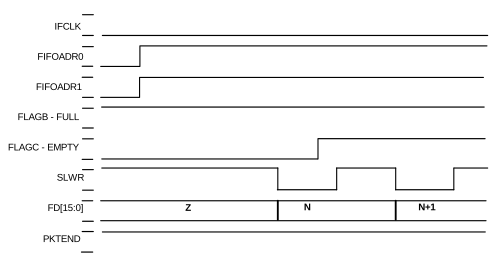
\includegraphics[width=.95\textwidth]{rdop_time}}
	\only<2>{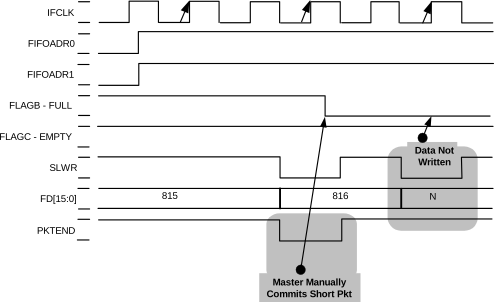
\includegraphics[width=.95\textwidth]{pktend_time}}
\end{frame}
\begin{frame}{Operaciones en la FIFO}
	\framesubtitle{Lectura Asíncrona}
	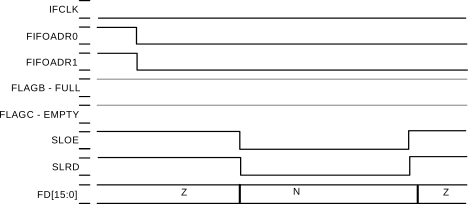
\includegraphics[width=.95\textwidth]{wrop_time}
\end{frame}

\begin{frame}{Máquina de estados algorítmica de la interfaz}
	\centering
	\begin{tikzpicture}[ask/.style = {diamond,text width=70,draw=black,align=center,aspect=2},
	scale=.41]
		\begin{scope}[transform shape,node distance=(1 and 4),>=latex,]
			\node[moore,text width=110] (inicio) [label=above right:inicio]{FIFOADR=$''$ZZ$''$\\FDATA=$''$ZZ$''$\\d\_recibido=d\_recibido\\SLOE=$'1'$\\SLRD=$'1'$\\SLWR=$'1'$};
		
			\node[ask] (vacio1) [below=of inicio]{FLAG\_Vacío};
				\draw[->] (inicio.south) -| (vacio1);
		%			\node[moore,text width=100] (lecdir) [below=of vacio1,label=above right:dirección] {FIFOADR=entrada\\SLOE=$'0'$\\SLRD=$'1'$\\SLWR=$'1'$};
		%			\draw[o->](vacio1.east) -- ($(vacio1.east)+(1,0)$);
		
			\node[moore,text width=110] (lecoe) [right=of vacio1,label=above right:dir\_lect] {FIFOADR=$''11''$\\FDATA=$''$ZZ$''$\\d\_recibido=FD\\SLOE=$'0'$\\SLRD=$'1'$\\SLWR=$'1'$};
				\draw[->] (vacio1.east) -- ($(vacio1.east)!0.5!(lecoe.west)$);
				\draw[->]($(vacio1.east)!0.5!(lecoe.west)$) |- ($(lecoe.north)+(0,1)$) -- (lecoe.north);
		
			\node[moore,text width=110](lecrd)[below=of lecoe,label=above right:lectura]{FIFOADR=$''11''$\\FDATA=$''$ZZ$''$\\D\_recibido=FD\\SLOE=$'0'$\\SLRD=$'0'$\\SLWR=$'1'$};
				\draw[->](lecoe) -- (lecrd);
		
			\node[ask] (vacio2)[below=of lecrd]{FLAG\_Vacío};
				\draw[->](lecrd) -- (vacio2);
				
				\draw[o->](vacio2.west) -| ($(lecoe.west)!.5!(vacio1.east)$);
				\draw[->](vacio2.east) -- ++(1.5,0) |- ($(inicio.north)+(0,1)$);
				\draw[->] ($(inicio.north)+(0,1)$) -- (inicio.north);
		
			\node[ask](enviar1)[below=of vacio1]{Enviar\_datos};
				\draw[o->](vacio1.south) --(enviar1.north);
		
		
			\node[ask] (lleno1) [below=of enviar1]{FLAG\_Lleno};
				\draw[->](enviar1) -- (lleno1);
		
			\node[moore,text width=110](escdir)[below=of lleno1,label=above left:dir\_escr]{FIFOADR=$''00''$\\FDATA=d\_a\_enviar\\d\_recibido=d\_recibido\\SLOE=$'1'$\\SLRD=$'1'$\\SLWR=$'1'$};
				\draw[->](lleno1) -- ($(lleno1.south)!0.5!(escdir.north)$);
				\draw[->]($(lleno1.south)!0.5!(escdir.north)$) -- (escdir);
		
		
			\node[ask](vacio3)[left=of vacio1]{FLAG\_Vacío};
				\draw[->](escdir.south)--($(escdir.south)+(0,-.5)$) -| ($(vacio3.east)+(1,0)$) |- ($(vacio3.north)+(0,1)$)-|(vacio3.north);
		
			\node[ask](enviar2)[below=of vacio3]{Enviar\_datos};
				\draw[o->](vacio3) -- (enviar2);
		
				\draw[o->] (enviar1.west) -- ($(enviar1.west)+(-1,0)$);
				\draw[->] ($(enviar1.west)-(1,0)$) -- ($(inicio.north -| enviar1.west)+(-1,1)$);
				\draw[->] ($(inicio.north -| enviar1.west)+(-1,1)$)--($(inicio.north)+(0,1)$);
				\draw[->] ($(inicio.north)+(0,1)$) -- (inicio.north);
				\draw[o->](lleno1.west) -| ($(enviar1.west)-(1,0)$);
				\draw[->](vacio3.west) -- ($(vacio3.west)+(-1,0)$);
				\draw[->]($(vacio3.west)+(-1,0)$) |- ($(inicio.north -| enviar1.west)+(-1,1)$);
		
			\node[ask](lleno2)[below=of enviar2]{FLAG\_Lleno};
			\node[moore,text width=110](escwr)[below=of lleno2,label=above left:escribir]{FIFOADR=$''00''$\\FDATA=d\_a\_enviar\\d\_recibido=d\_recibido\\SLOE=$'1'$\\SLRD=$'1'$\\SLWR=$'0'$};
				\draw[->](lleno2) -- (escwr);
				\draw[o->](lleno2.west) -| ($(enviar2.west)+(-1,0)$);
				\draw[->](enviar2)--(lleno2);
				\draw[o->](enviar2)--($(enviar2.west)+(-1,0)$);
				\draw[->]($(enviar2.west)+(-1,0)$) -- ($(vacio3.west)+(-1,0)$);
				\draw[->](escwr) -- ($(escwr.south)+(0,-1)$) -| ($(escdir.east)+(1,0)$) |- ($(lleno1.south)!0.5!(escdir.north)$);
		\end{scope}
	\end{tikzpicture}
\end{frame}

\begin{frame}{Verificación Funcional}
%	\only<1>{
%		\centering
%		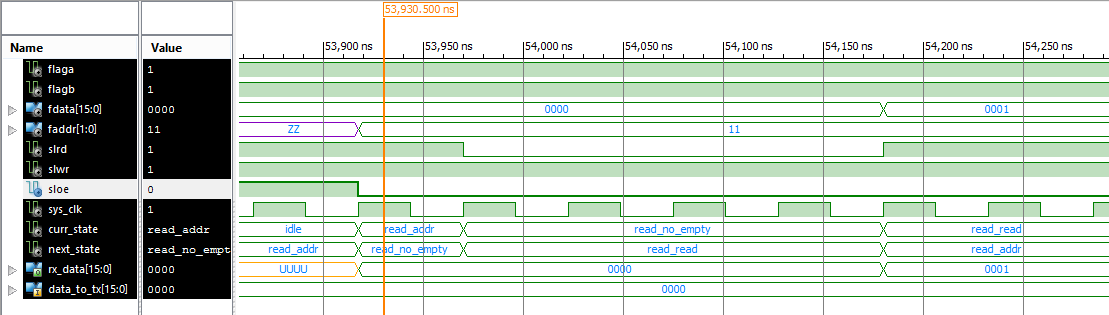
\includegraphics[width=\textwidth]{tb_if_rd_mef}\\
%		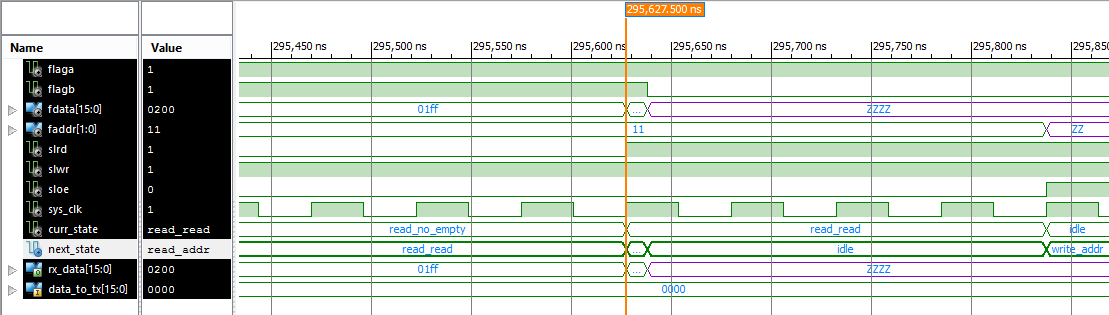
\includegraphics[width=\textwidth]{tb_if_rd_end}
%	}
%	\only<2>{
		\framesubtitle{Operación de escritura}
		\centering
		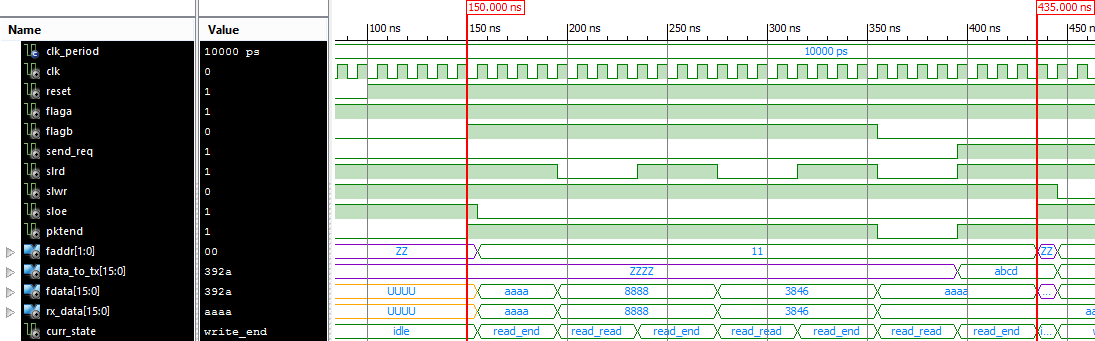
\includegraphics[width=\textwidth]{mef_tb_lect_marcas}
%	}
\end{frame}
\begin{frame}{Verificación Funcional}
	\framesubtitle{Operación de escritura}
	\centering
		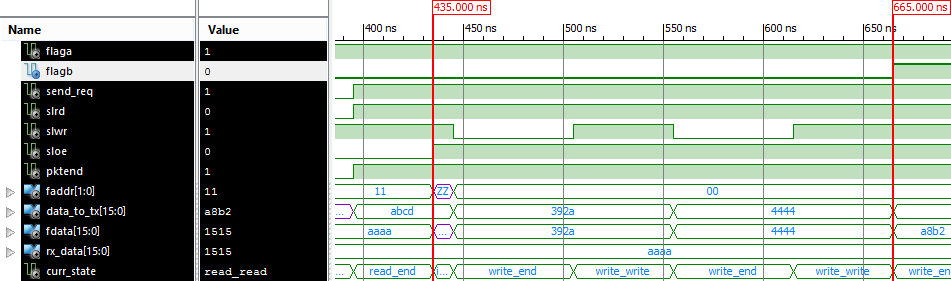
\includegraphics[width=\textwidth]{mef_tb_escr_marcas}\\
		\vfill
		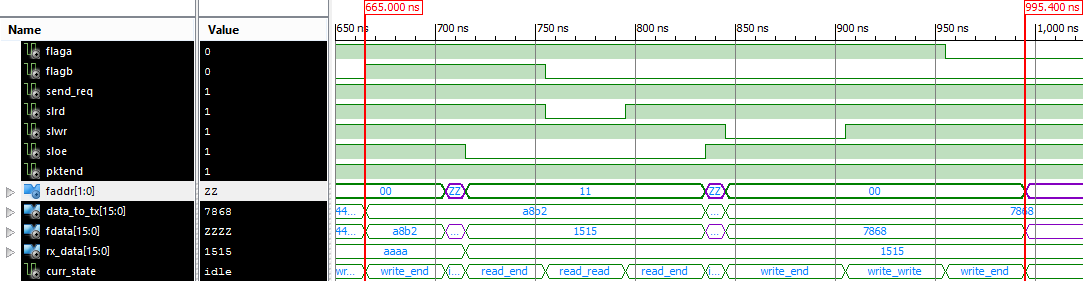
\includegraphics[width=\textwidth]{mef_tb_full}
\end{frame}

%\begin{frame}{Implementación de la máquina de estados de la interfaz}
%	\scriptsize{
%		\only<1>{
%			\lstinputlisting[language=VHDL,firstline=20,lastline=28]{./codes/fx2lp_interface.vhd}
%			}
%		\only<2>{
%			\lstinputlisting[language=VHDL,firstline=29,lastline=48]{./codes/fx2lp_interface.vhd}
%		}
%		\only<3>{
%			\lstinputlisting[language=VHDL,firstline=50,lastline=67]{./codes/fx2lp_interface.vhd}
%		}
%		\only<4>{
%			\lstinputlisting[language=VHDL,firstline=69,lastline=76]{./codes/fx2lp_interface.vhd}
%		}
%		\only<5>{
%			\lstinputlisting[language=VHDL,firstline=78,lastline=92]{./codes/fx2lp_interface.vhd}
%		}
%		\only<6>{
%			\lstinputlisting[language=VHDL,firstline=94,lastline=113]{./codes/fx2lp_interface.vhd}
%		}
%		\only<7-8>{
%			\lstinputlisting[language=VHDL,firstline=115,lastline=118]{./codes/fx2lp_interface.vhd}}
%		\only<7>{
%			\begin{columns}[t]
%				\begin{column}{.5\textwidth}
%					\lstinputlisting[language=VHDL,firstline=119,lastline=134]{./codes/fx2lp_interface.vhd}
%				\end{column}				\begin{column}{.5\textwidth}
%					\lstinputlisting[language=VHDL,firstline=135,lastline=146]{./codes/fx2lp_interface.vhd}
%				\end{column}
%			\end{columns}
%		}
%		\only<8>{
%			\begin{columns}[t]
%				\begin{column}{.5\textwidth}
%					\lstinputlisting[language=VHDL,firstline=147,lastline=158]{./codes/fx2lp_interface.vhd}
%				\end{column}
%				\begin{column}{.5\textwidth}
%				\end{column}
%			\end{columns}
%			\lstinputlisting[language=VHDL,firstline=159,lastline=160]{./codes/fx2lp_interface.vhd}
%		}
%		\only<9>{
%			\lstinputlisting[language=VHDL,firstline=162,lastline=176]{./codes/fx2lp_interface.vhd}
%		}
%		\only<10>{
%			\lstinputlisting[language=VHDL,firstline=178,lastline=193]{./codes/fx2lp_interface.vhd}
%		}		
%		\only<11>{
%			\lstinputlisting[language=VHDL,firstline=195,lastline=206]{./codes/fx2lp_interface.vhd}
%		}
%	}
%\end{frame}
%\begin{frame}{Instanciación de la interfaz en el top}
%	\tiny{
%		\only<1>{
%			\lstinputlisting[language=VHDL,firstline=7,lastline=34]{./codes/fx2lp_interface_top.vhd}
%		}
%		\only<2>{
%			\lstinputlisting[language=VHDL,firstline=36,lastline=61]{./codes/fx2lp_interface_top.vhd}
%		}
%	}
%\end{frame}
%\begin{frame}{Maquinas de estado hacia la memoria FIFO interna}
%	\begin{columns}
%		\begin{column}{.5\textwidth}
%			\centering
%			\begin{tikzpicture}[scale=.53]
%				\begin{scope}[transform shape,node distance=1,>=latex]
%					\node[moore] (idle) {--idle:\\RE\_EN='0';};
%					\node[node distance=.6](aux0)[above=of idle]{};
%					\node[ask]	(pr1)	[below=of idle]{\tiny{SLWR='0'-$>$'1'}}
%						edge[<-] (idle);
%					\node[ask] (pr2) [below=of pr1]{\scriptsize{FIFO\_empty='1'}};
%					\node[node distance=.8](aux1)[left=of pr1]{};
%					\draw[->] (pr1) -- node[left] {Si} (pr2);
%					\draw[->] (pr1) -- node[above,near start]{No} (aux1.base);
%					\draw[->] (aux1.base) |- (aux0.base) -- (idle);
%					
%					\node[moore](rden)[below=of pr2]{--read enable:\\RD\_EN='1'};
%					\node[node distance=.8] (aux2) [left=of pr2] {};
%					\draw[->] (pr2) -- node[above,near start]{Si} (aux2.base);
%					\draw[->] (pr2) -- node[left,near start] {No} (rden);
%					\draw[->] (aux2.base) -- (aux1.base);
%					
%					\node[node distance=.8] (aux3) [below=of rden]{};
%					\draw[->] (rden) -- (aux3.base) -| (aux2.base); 
%				\end{scope}
%			\end{tikzpicture}
%		\end{column}
%		\begin{column}{.5\textwidth}
%			\centering
%			\begin{tikzpicture}[scale=.5]
%				\begin{scope}[transform shape,node distance=1,>=latex]
%					\node[moore] (idle) {--idle:\\WR\_EN='0';};
%					\node[node distance=.6](aux0)[above=of idle]{};
%					\node[ask]	(pr1)	[below=of idle]{\tiny{SLRD='0'-$>$'1'}}
%						edge[<-] (idle);
%					\node[ask] (pr2) [below=of pr1]{\scriptsize{FIFO\_FULL='1'}};
%					\node[node distance=.8](aux1)[left=of pr1]{};
%					\draw[->] (pr1) -- node[left] {Si} (pr2);
%					\draw[->] (pr1) -- node[above,near start]{No} (aux1.base);
%					\draw[->] (aux1.base) |- (aux0.base) -- (idle);
%					
%					\node[moore](rden)[below=of pr2]{--write enable:\\WR\_EN='1'};
%					\node[node distance=.8] (aux2) [left=of pr2] {};
%					\draw[->] (pr2) -- node[above,near start]{Si} (aux2.base);
%					\draw[->] (pr2) -- node[left,near start] {No} (rden);
%					\draw[->] (aux2.base) -- (aux1.base);
%					
%					\node[node distance=.8] (aux3) [below=of rden]{};
%					\draw[->] (rden) -- (aux3.base) -| (aux2.base); 
%				\end{scope}
%			\end{tikzpicture}
%		\end{column}
%	\end{columns}
%\end{frame}
